\documentclass[12pt,english,dvipsnames,aspectratio=169,handout]{beamer}\usepackage[]{graphicx}\usepackage[]{xcolor}
% maxwidth is the original width if it is less than linewidth
% otherwise use linewidth (to make sure the graphics do not exceed the margin)
\makeatletter
\def\maxwidth{ %
  \ifdim\Gin@nat@width>\linewidth
    \linewidth
  \else
    \Gin@nat@width
  \fi
}
\makeatother

\definecolor{fgcolor}{rgb}{0.345, 0.345, 0.345}
\newcommand{\hlnum}[1]{\textcolor[rgb]{0.686,0.059,0.569}{#1}}%
\newcommand{\hlstr}[1]{\textcolor[rgb]{0.192,0.494,0.8}{#1}}%
\newcommand{\hlcom}[1]{\textcolor[rgb]{0.678,0.584,0.686}{\textit{#1}}}%
\newcommand{\hlopt}[1]{\textcolor[rgb]{0,0,0}{#1}}%
\newcommand{\hlstd}[1]{\textcolor[rgb]{0.345,0.345,0.345}{#1}}%
\newcommand{\hlkwa}[1]{\textcolor[rgb]{0.161,0.373,0.58}{\textbf{#1}}}%
\newcommand{\hlkwb}[1]{\textcolor[rgb]{0.69,0.353,0.396}{#1}}%
\newcommand{\hlkwc}[1]{\textcolor[rgb]{0.333,0.667,0.333}{#1}}%
\newcommand{\hlkwd}[1]{\textcolor[rgb]{0.737,0.353,0.396}{\textbf{#1}}}%
\let\hlipl\hlkwb

\usepackage{framed}
\makeatletter
\newenvironment{kframe}{%
 \def\at@end@of@kframe{}%
 \ifinner\ifhmode%
  \def\at@end@of@kframe{\end{minipage}}%
  \begin{minipage}{\columnwidth}%
 \fi\fi%
 \def\FrameCommand##1{\hskip\@totalleftmargin \hskip-\fboxsep
 \colorbox{shadecolor}{##1}\hskip-\fboxsep
     % There is no \\@totalrightmargin, so:
     \hskip-\linewidth \hskip-\@totalleftmargin \hskip\columnwidth}%
 \MakeFramed {\advance\hsize-\width
   \@totalleftmargin\z@ \linewidth\hsize
   \@setminipage}}%
 {\par\unskip\endMakeFramed%
 \at@end@of@kframe}
\makeatother

\definecolor{shadecolor}{rgb}{.97, .97, .97}
\definecolor{messagecolor}{rgb}{0, 0, 0}
\definecolor{warningcolor}{rgb}{1, 0, 1}
\definecolor{errorcolor}{rgb}{1, 0, 0}
\newenvironment{knitrout}{}{} % an empty environment to be redefined in TeX

\usepackage{alltt}
\usepackage{fontspec}
\setsansfont[Mapping=tex-text]{Fira Sans}
\setcounter{secnumdepth}{4}
\setcounter{tocdepth}{4}
\usepackage[normalem]{ulem}
\usepackage[T1]{fontenc}
\usepackage{dcolumn}
\usepackage{booktabs}
\usepackage{setspace}
\makeatletter
\usetheme{metropolis}
\setbeamertemplate{frame footer}{Bosancianu | Schaub | Hertie School}
\setbeamerfont{page number in head/foot}{size=\tiny}
\setbeamercolor{footline}{fg=gray}
\usepackage{xcolor}
\usepackage{tikz}
\usetikzlibrary{arrows, positioning}
\usepackage[labelformat=empty]{caption}
% For table captions in Beamer
\usepackage[sectionbib]{apacite}
\renewcommand{\bibliographytypesize}{\footnotesize}
\makeatletter
\let\st@rtbibsection\@bibnewpage
\let\st@rtbibchapter\@bibnewpage
\makeatother
\usepackage{amsmath, mathtools}
\usepackage{xunicode}
\usepackage{hyperref}
\graphicspath{{./figures/}} 
% Defines a checkmark
\def\checkmark{\tikz\fill[scale=0.4,color=orange](0,.35) -- (.25,0) -- (1,.7) -- (.25,.15) -- cycle;}
% boxes
\def\boxitorange#1{%
	\smash{\color{orange}\fboxrule=1pt\relax\fboxsep=2pt\relax%
		\llap{\rlap{\fbox{\vphantom{0}\makebox[#1]{}}}~}}\ignorespaces
}
\def\boxitblue#1{%
	\smash{\color{blue}\fboxrule=1pt\relax\fboxsep=2pt\relax%
		\llap{\rlap{\fbox{\vphantom{0}\makebox[#1]{}}}~}}\ignorespaces
}
\newcommand{\indep}{\perp \!\!\!\! \perp}
\setbeamertemplate{itemize items}{\checkmark}
\usepackage{multirow}
\usepackage{subcaption}
\hypersetup{pdfauthor={Bosancianu and Schaub},
	pdftitle={Statistical Modeling and Causal Inference with R},
	pdfsubject={Week 4: Causal Graphs},
	pdfkeywords={Berlin, Hertie, 2020, week 4}}
\title{\textsc{Statistical Modeling and Causal Inference with R}}
\subtitle{Week 4: Causal Graphs}
\date{September 28, 2020}
\author{Manuel Bosancianu \hfill Max Schaub}
\institute{Hertie School}
\IfFileExists{upquote.sty}{\usepackage{upquote}}{}
\begin{document}
\maketitle

\section{d-separation}




\begin{frame}
	\frametitle{Canonical configurations: confounders}
	\begin{figure}
		\centering
		\begin{tikzpicture}[->,
			>=stealth',
			shorten >=1pt,
			auto,
			thick]
			
			\draw[fill=black, draw=black] (0,0) circle (0.6ex) node (a) [below, yshift=-0.2cm] {\large\texttt{D}};
			\draw[fill=black, draw=black] (2,0) circle (0.6ex) node (b) [below, yshift=-0.2cm] {\large\texttt{Y}};
			\draw[fill=black, draw=black] (1,1.5) circle (0.6ex) node (b) [above, yshift=0.2cm] {\large\texttt{C}};
			\draw[->, orange] (0.12,0) -- (1.92,0);
			\draw[->, black] (1,1.5) -- (0.05,0.1);
			\draw[->, black] (1.05,1.38) -- (1.94,0.06);
		\end{tikzpicture}
	\end{figure}
	
	$D \leftarrow C \rightarrow Y$ is an \textcolor{orange}{open} back-door path (\texttt{C} is not a collider).\bigskip
	
	\textcolor{orange}{Solution}: condition on \texttt{C} to close the path.
	
	\begin{equation}
		Y_i = \beta_0 + \beta_1D_i + \beta_2C_i + \epsilon_i
	\end{equation}
	
\end{frame}


\begin{frame}
	\frametitle{Canonical configurations: mediators}
	\begin{figure}
		\centering
		\begin{tikzpicture}[->,
			>=stealth',
			shorten >=1pt,
			auto,
			thick]
			
			\draw[fill=black, draw=black] (0,0.75) circle (0.8ex) node (a) [below, yshift=-0.2cm] {\large\texttt{D}};
			\draw[fill=black, draw=black] (2,0.75) circle (0.8ex) node (b) [below, yshift=-0.2cm] {\large\texttt{C}};
			\draw[fill=black, draw=black] (4,0.75) circle (0.8ex) node (b) [below, yshift=-0.2cm] {\large\texttt{Y}};
			\draw[->, black] (0,0.75) -- (1.92,0.75);
			\draw[->, black] (2,0.75) -- (3.92,0.75);
		\end{tikzpicture}
	\end{figure}
	
	$D \rightarrow C \rightarrow Y$: causal path between treatment and outcome.\bigskip
	
	\textcolor{orange}{Solution}: do not condition on C, to keep the path open.\bigskip
	
	Rules:
	
	\begin{itemize}
		\item close all non-causal paths linking \texttt{D} to \texttt{Y}
		\item do not close any causal path between \texttt{D} and \texttt{Y}
	\end{itemize}
	
	
\end{frame}




\begin{frame}
	\frametitle{Canonical configurations: colliders}
	\begin{figure}
		\centering
	\begin{tikzpicture}[->,
		>=stealth',
		shorten >=1pt,
		auto,
		thick]
		
		\draw[fill=black, draw=black] (0,0) circle (0.8ex) node (a) [below, yshift=-0.2cm] {\large\texttt{D}};
		\draw[fill=black, draw=black] (2,0) circle (0.8ex) node (b) [below, yshift=-0.2cm] {\large\texttt{Y}};
		\draw[fill=black, draw=black] (1,1.5) circle (0.8ex) node (b) [above, yshift=0.2cm] {\large\texttt{C}};
		\draw[->, orange] (0.15,0) -- (1.92,0);
		\draw[->, black] (0.05,0.12) -- (0.95,1.45);
		\draw[->, black] (1.95,0.12) -- (1.05,1.45);
	\end{tikzpicture}
	\end{figure}
	
	$D \rightarrow C \leftarrow Y$: noncausal path between treatment and outcome.\bigskip
	
	\textcolor{orange}{Solution}: do not condition on C, as path is closed already.\bigskip
	
	Don't condition on a descendant of a collider, either \cite[p.~44-45]{pearl_causal_2016}.
	
\end{frame}


\begin{frame}
  \frametitle{Truncation in data}
  Is there a negative relationship between talent and beauty among actors?\bigskip
  
  \pause
  
  Strong argument for "no"; spurious relationship.\bigskip


\begin{knitrout}
\definecolor{shadecolor}{rgb}{0.969, 0.969, 0.969}\color{fgcolor}

{\centering \includegraphics[width=\maxwidth]{figure/r_generate-data-1} 

}


\end{knitrout}

\end{frame}


\begin{frame}
  \frametitle{Selection by cutoff}
  
  \begin{equation}
  \centering
  Star\; potential_i = Beauty_i + Talent_i
  \end{equation}\bigskip
  
  Top 15\% succeed as actors.
  
  \pause
  
  \begin{figure}
		\centering
	\begin{tikzpicture}[->,
				>=stealth',
				shorten >=1pt,
				auto,
				thick]
				\node at (2,2) (a) [text width = 1.75cm] {\footnotesize Movie star};
				\node at (0,0) (b) [text width = 1cm] {\footnotesize Talent};
				\node at (4,0) (c) [text width = 1cm] {\footnotesize Beauty};
				\draw[->, black] (b) -- (a);
				\draw[->, black] (c) -- (a);
			\end{tikzpicture}
	\end{figure}

  
\end{frame}

\begin{frame}
  \frametitle{Effects of conditioning on collider}
  
\begin{knitrout}
\definecolor{shadecolor}{rgb}{0.969, 0.969, 0.969}\color{fgcolor}

{\centering \includegraphics[width=\maxwidth]{figure/r_actors-truncation-1} 

}


\end{knitrout}
  
\end{frame}


\begin{frame}
  \frametitle{Effects of conditioning on collider}
  
\begin{knitrout}
\definecolor{shadecolor}{rgb}{0.969, 0.969, 0.969}\color{fgcolor}

{\centering \includegraphics[width=\maxwidth]{figure/r_conditioned-trend-1} 

}


\end{knitrout}

Negative relationship, when none exists in population.
  
\end{frame}


\begin{frame}
	\frametitle{Strategy for \textit{d}-separation}
	A few simple steps \cite[p.~73]{cunningham_causal_2021}:
	
	\begin{enumerate}
		\item write down all paths between \texttt{D} and \texttt{Y}
		
		\item identify open/closed back-door paths (any confounders or colliders?)
		
		\item find conditioning strategy that closes all open back-doors
	\end{enumerate}
	
	Last step is not always possible.
		
\end{frame}


\section{Practice}

\begin{frame}
	\frametitle{Practice \#1}

  \begin{minipage}{0.47\linewidth}

  \begin{figure}
  		\centering
	\begin{tikzpicture}[->,
				>=stealth',
				shorten >=1pt,
				auto,
				thick]
				\node at (0,0) (x) [text width = 0.5cm, align=center] {\textcolor{orange}{X}};
				\node at (4,0) (y) [text width = 0.5cm, align=center] {\textcolor{orange}{Y}};
				\node at (2,2) (b) [text width = 0.5cm, align=center] {\textcolor{orange}{B}};
				\node at (2,0.7) (a) [text width = 0.5cm, align=center] {\textcolor{orange}{A}};
				\draw[->, black] (x) -- (y);
				\draw[->, black] (b) -- (y);
				\draw [->, black] (b) -- (x);
				\draw [->, black] (x) -- (a);
				\draw [->, black] (b) -- (a);
			\end{tikzpicture}
			\caption{Estimate $X \rightarrow Y$}
  \end{figure}
  
  \end{minipage}
  \pause
  \begin{minipage}{0.47\linewidth}
  
  One back-door path:
  
  $X \leftarrow B \rightarrow Y$.
  
  \end{minipage}
		
\end{frame}


\begin{frame}
	\frametitle{Practice \#2}

  \begin{minipage}{0.47\linewidth}

  \begin{figure}
  		\centering
	\begin{tikzpicture}[->,
				>=stealth',
				shorten >=1pt,
				auto,
				thick]
				\node at (0,0) (x) [text width = 0.5cm, align=center] {\textcolor{orange}{X}};
				\node at (4,0) (y) [text width = 0.5cm, align=center] {\textcolor{orange}{Y}};
				\node at (0,2) (a) [text width = 0.5cm, align=center] {\textcolor{orange}{A}};
				\node at (4,2) (c) [text width = 0.5cm, align=center] {\textcolor{orange}{C}};
				\node at (2,1) (b) [text width = 0.5cm, align=center] {\textcolor{orange}{B}};
				\draw[->, black] (a) -- (x);
				\draw[->, black] (a) -- (b);
				\draw [->, black] (c) -- (b);
				\draw [->, black] (c) -- (y);
			\end{tikzpicture}
			\caption{Estimate $X \rightarrow Y$}
  \end{figure}
  
  \end{minipage}
  \pause
  \begin{minipage}{0.47\linewidth}
  
  "M-bias."\bigskip
  
  One back-door path:
  
  $X \leftarrow A \rightarrow B \leftarrow C \rightarrow Y$\bigskip
  
  No need to control for any variable.
  
  \end{minipage}
		
\end{frame}



\begin{frame}
	\frametitle{Practice \#3}

  \begin{minipage}{0.47\linewidth}

  \begin{figure}
  		\centering
	\begin{tikzpicture}[->,
				>=stealth',
				shorten >=1pt,
				auto,
				thick]
				\node at (0,0) (x) [text width = 0.5cm, align=center] {\textcolor{orange}{X}};
				\node at (4,0) (y) [text width = 0.5cm, align=center] {\textcolor{orange}{Y}};
				\node at (0,2) (a) [text width = 0.5cm, align=center] {\textcolor{orange}{A}};
				\node at (4,2) (c) [text width = 0.5cm, align=center] {\textcolor{orange}{C}};
				\node at (2,1) (b) [text width = 0.5cm, align=center] {\textcolor{orange}{B}};
				\draw[->, black] (a) -- (x);
				\draw[->, black] (a) -- (b);
				\draw [->, black] (c) -- (b);
				\draw [->, black] (c) -- (y);
				\draw [->, black] (b) -- (x);
				\draw [->, black] (x) -- (y);
			\end{tikzpicture}
			\caption{Estimate $X \rightarrow Y$}
  \end{figure}
  
  \end{minipage}
  \pause
  \begin{minipage}{0.47\linewidth}
  
  Two back-door paths:
  
  $X \leftarrow A \rightarrow B \leftarrow C \rightarrow Y$
  
  $X \leftarrow B \leftarrow C \rightarrow Y$\bigskip
  
  \pause
  
  Either control for $B$ \& either $A$ or $C$, or just for $C$.
  
  
  \end{minipage}
		
\end{frame}


\section{Racially-biased policing}

\begin{frame}
  \frametitle{The setup}
  \textcolor{orange}{Question}: \pause Can commonly-used administrative data on police stops reveal racially-biased policing?\bigskip
  
  \pause
  
  \textcolor{orange}{Fundamental} problem: Impossible to detect if administrative records suffer from bias.\bigskip
  
  Race also influences whether police decide to stop a person (only a stop triggers a report being filled in).
  
\end{frame}


\begin{frame}
  \frametitle{The setup}
  Studying racial bias in policing: "inherently causal inquiry".\bigskip
  
  \textcolor{orange}{Counterfactual}: \pause What would be the outcome if an individual of different race would encounter police in same location, time, for same criminal conduct\dots
  
  Multiple estimands: $ATE$ or $ATE_{M=1}$.
  
\end{frame}


\begin{frame}
  \frametitle{The setup}
  Studying racial bias in policing: "inherently causal inquiry".\bigskip
  
  \textcolor{orange}{Counterfactual}: \pause What would be the outcome if an individual of different race would encounter police in same location, time, for same criminal conduct\dots
  
  Multiple estimands: $ATE$ or $ATE_{M=1}$.
  
\end{frame}


\begin{frame}
  \frametitle{DAG}
  
  \begin{figure}
		\centering
		\begin{spacing}{0.5}
	\begin{tikzpicture}[->,
				>=stealth',
				shorten >=1pt,
				auto,
				thick]
				\node at (0,0) (d) [text width = 1.2cm, align=center] {\footnotesize Minority (\textcolor{orange}{D})};
				\node at (3,0) (m) [text width = 1cm, align=center] {\footnotesize Stop (\textcolor{orange}{M})};
				\node at (6,0) (y) [text width = 1cm, align=center] {\footnotesize Force (\textcolor{orange}{Y})};
				\node at (4.5,2) (u) [text width = 1.3cm, align=center] {\footnotesize Suspicion (\textcolor{orange}{U})};
				\draw[->, black] (d) -- (m);
				\draw[->, black] (m) -- (y);
				\draw[->, black] (u) -- (m);
				\draw[->, black] (u) -- (y);
				\draw [->, black] (d.south) to [out=300,in=240] (y.south);
			\end{tikzpicture}
			\end{spacing}
	\end{figure}
  
  $D \in \{0;1\}$, with $1$ designating "minority".
  
  Unobservables include: sense of threat, suspicion.
  
  
\end{frame}




\begin{frame}
  \frametitle{DAG}
  
  \begin{figure}[scale = 0.4]
		\centering
		\begin{spacing}{0.5}
	\begin{tikzpicture}[->,
				>=stealth',
				shorten >=1pt,
				auto,
				thick]
				\node at (0,0) (d) [text width = 1.2cm, align=center] {\footnotesize Minority (\textcolor{orange}{D})};
				\node at (3,0) (m) [text width = 1cm, align=center] {\footnotesize Stop (\textcolor{orange}{M})};
				\node at (6,0) (y) [text width = 1cm, align=center] {\footnotesize Force (\textcolor{orange}{Y})};
				\node at (4.5,2) (u) [text width = 1.3cm, align=center] {\footnotesize Suspicion (\textcolor{orange}{U})};
				\draw[->, black] (d) -- (m);
				\draw[->, black] (m) -- (y);
				\draw[->, black] (u) -- (m);
				\draw[->, black] (u) -- (y);
				\draw [->, black] (d.south) to [out=300,in=240] (y.south);
			\end{tikzpicture}
			\end{spacing}
	\end{figure}
  
  \begin{equation}
  \centering
  ITE_i = Y_i^1(M_i^1) - Y_i^0(M_i^0)
  \end{equation}
  
\end{frame}


\begin{frame}
  \frametitle{Difficulty with ATE}
  
  \begin{equation}
  \centering
  ATE = E[Y_i^1(M_i^1)] - E[Y_i^0(M_i^0)]
  \end{equation}
  
  Quantity depends on:
  
  \begin{itemize}
  \item minorities are stopped at differential rates
  \item minorities are subjected to violence at differential rates
  \end{itemize}
  
\end{frame}


\begin{frame}
  \frametitle{Partial illustration \cite{bronner_why_2020}}
  
  \begin{figure}
  \centering
  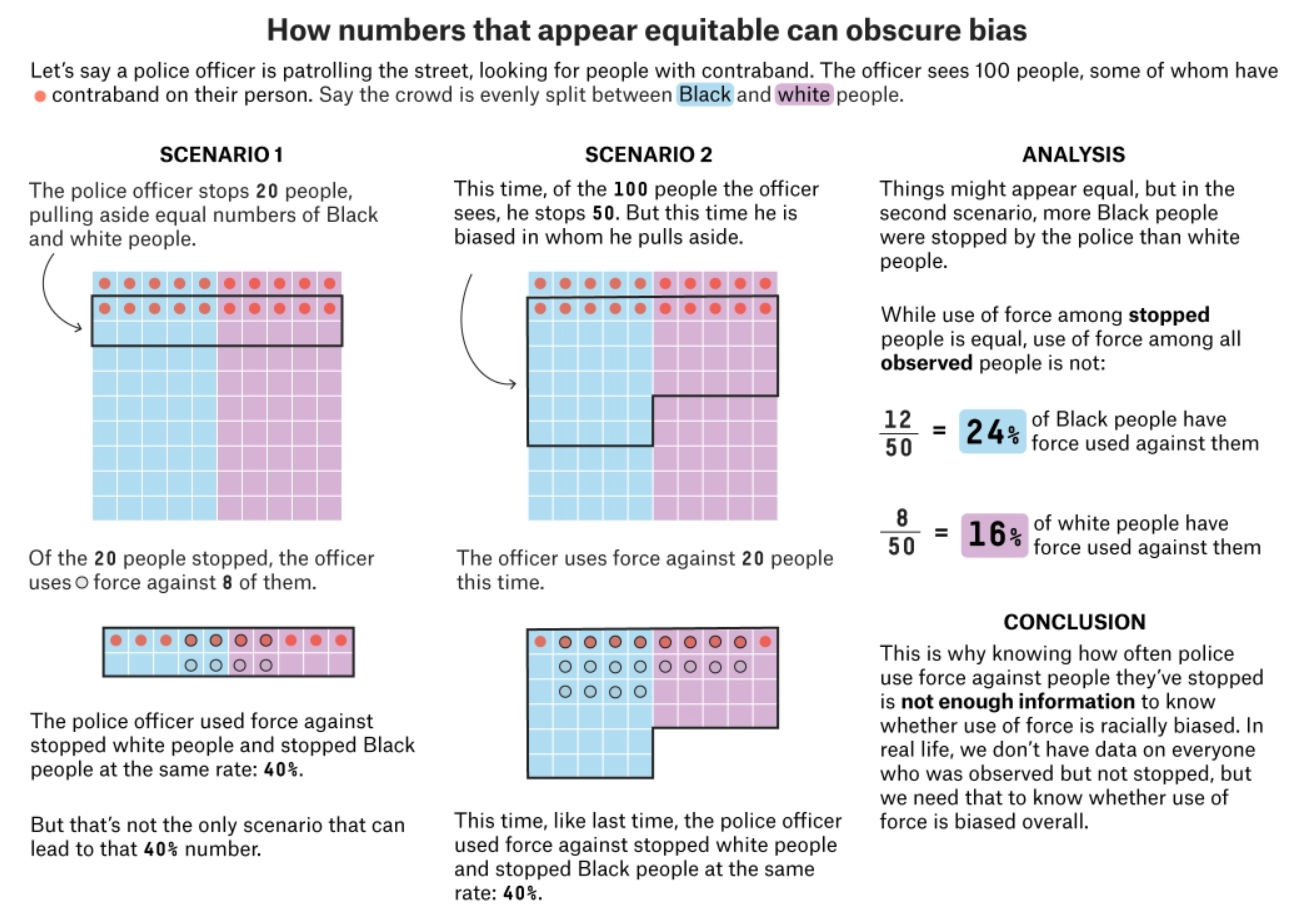
\includegraphics[scale = 0.33]{../04-figures/04/04-09}
  \end{figure}
\end{frame}


\begin{frame}
  \frametitle{What is this about?}
  
  \begin{figure}[scale = 0.4]
		\centering
		\begin{spacing}{0.5}
	\begin{tikzpicture}[->,
				>=stealth',
				shorten >=1pt,
				auto,
				thick]
				\node at (0,0) (d) [text width = 1.2cm, align=center] {\footnotesize Minority (\textcolor{orange}{D})};
				\node at (3,0) (m) [text width = 1cm, align=center] {\footnotesize Stop (\textcolor{orange}{M})};
				\node at (6,0) (y) [text width = 1cm, align=center] {\footnotesize Force (\textcolor{orange}{Y})};
				\node at (4.5,2) (u) [text width = 1.3cm, align=center] {\footnotesize Suspicion (\textcolor{orange}{U})};
				\draw[->, orange] (d) -- (m);
				\draw[->, black] (m) -- (y);
				\draw[->, orange] (u) -- (m);
				\draw[->, black] (u) -- (y);
				\draw [->, black] (d.south) to [out=300,in=240] (y.south);
			\end{tikzpicture}
			\end{spacing}
	\end{figure}
	
	\pause
	
	\textcolor{orange}{Collider bias}: police records condition on a collider, by recording only stops that are impacted themselves by race.
  
\end{frame}



\begin{frame}
  \frametitle{DAG}
  
  \begin{figure}[scale = 0.4]
		\centering
		\begin{spacing}{0.5}
	\begin{tikzpicture}[->,
				>=stealth',
				shorten >=1pt,
				auto,
				thick]
				\node at (0,0) (d) [text width = 1.2cm, align=center] {\footnotesize Minority (\textcolor{orange}{D})};
				\node at (3,0) (m) [text width = 1cm, align=center] {\footnotesize Stop (\textcolor{orange}{M})};
				\node at (6,0) (y) [text width = 1cm, align=center] {\footnotesize Force (\textcolor{orange}{Y})};
				\node at (4.5,2) (u) [text width = 1.3cm, align=center] {\footnotesize Suspicion (\textcolor{orange}{U})};
				\draw[->, black] (d) -- (m);
				\draw[->, black] (m) -- (y);
				\draw[->, black] (u) -- (m);
				\draw[->, black] (u) -- (y);
				\draw [->, black] (d.south) to [out=300,in=240] (y.south);
			\end{tikzpicture}
			\end{spacing}
	\end{figure}
  
  \begin{equation}
  \centering
  Naive = \hat{\delta} = E[Y_i^1 | D_i=1, M_i=1] - E[Y_i^0 | D_i=0, M_i=1]
  \end{equation}
  
  
\end{frame}



\begin{frame}
  \frametitle{Strata of contexts}
  
  \begin{figure}
  \begin{subfigure}{0.47\linewidth}
  \centering
  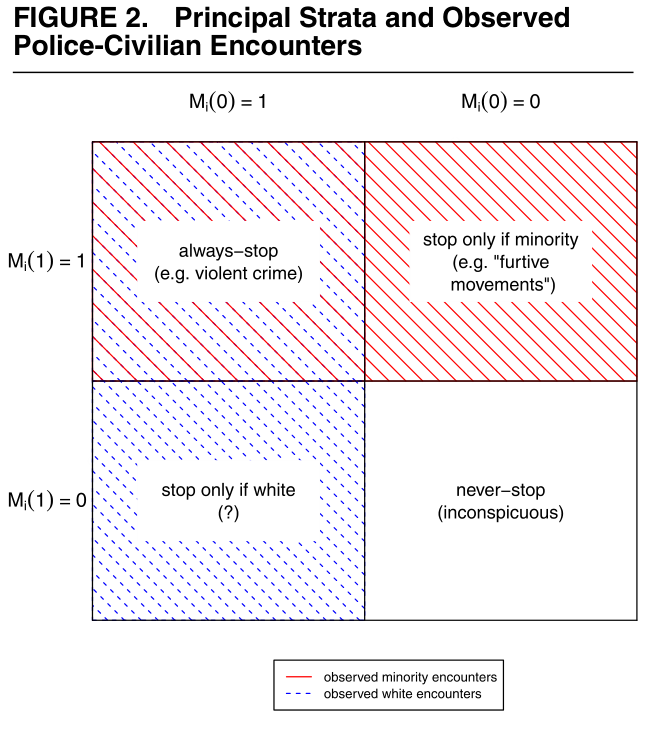
\includegraphics[scale = 0.35]{../04-figures/04/04-07}
  \end{subfigure}
  \begin{subfigure}{0.47\linewidth}
  \centering
  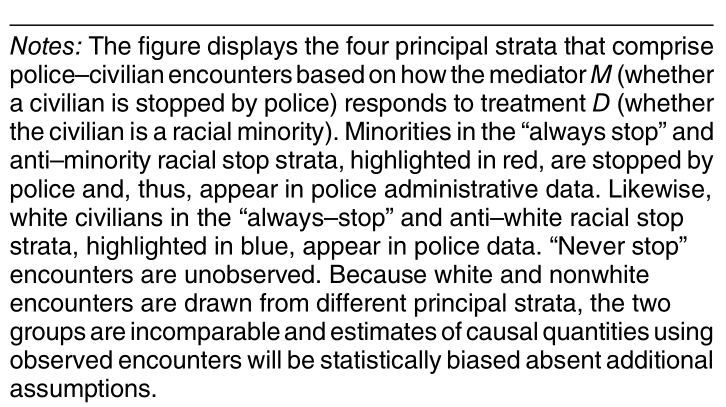
\includegraphics[scale = 0.35]{../04-figures/04/04-08}
  \end{subfigure}
  \end{figure}
  
  
\end{frame}


\begin{frame}
  \frametitle{Assumptions needed for $NATE=ATE$}
  
  \begin{minipage}{0.47\linewidth}
  \begin{equation}
  \centering
  M_i(d) \indep D_i|X_i
  \end{equation}
  After controlling for contextual factors (neighborhoods, police practices), race is independent of encounters.\bigskip
  
  \pause
  
  Can't be tested without data from "non-stops".
  \end{minipage}
  \pause
  \begin{minipage}{0.47\linewidth}

  \begin{figure}
  		\centering
	\begin{tikzpicture}[->,
				>=stealth',
				shorten >=1pt,
				auto,
				thick]
				\node at (0,0) (d) [text width = 0.5cm, align=center] {\textcolor{orange}{D}};
				\node at (2,0) (m) [text width = 0.5cm, align=center] {\textcolor{orange}{M}};
				\node at (4,0) (y) [text width = 0.5cm, align=center] {\textcolor{orange}{Y}};
				\node at (1,1) (w) [text width = 0.5cm, align=center] {\textcolor{orange}{W}};
				\draw[->, black] (d) -- (m);
				\draw[->, black] (m) -- (y);
				\draw[->, black] (w) -- (d);
				\draw[->, black] (w) -- (m);
				\draw [->, black] (d.south) to [out=300,in=240] (y.south);
			\end{tikzpicture}
			\caption{Assumption violation}
  \end{figure}
  \end{minipage}

\end{frame}


\begin{frame}
  \frametitle{Assumptions needed for $NATE=ATE$}
  
  \begin{equation}
  \centering
  Y_i(d,m) \indep D_i|M_{0i}=m', M_{1i}=m'', X_i
  \end{equation}
  
  \begin{minipage}{0.47\linewidth}
  
  A contextual factor shaped by race, and which influences violence, needs to be controlled for.\bigskip
  
  The 2 assumptions: "treatment ignorability".
  \end{minipage}
  \pause
  \begin{minipage}{0.47\linewidth}

  \begin{figure}
  		\centering
	\begin{tikzpicture}[->,
				>=stealth',
				shorten >=1pt,
				auto,
				thick]
				\node at (0,0) (d) [text width = 0.5cm, align=center] {\textcolor{orange}{D}};
				\node at (2,0) (m) [text width = 0.5cm, align=center] {\textcolor{orange}{M}};
				\node at (4,0) (y) [text width = 0.5cm, align=center] {\textcolor{orange}{Y}};
				\node at (2,2) (v) [text width = 0.5cm, align=center] {\textcolor{orange}{V}};
				\draw[->, black] (d) -- (m);
				\draw[->, black] (m) -- (y);
				\draw [->, black] (v.west) to [out=180,in=90] (d.north);
				\draw [->, black] (v.east) to [out=0,in=90] (y.north);
				\draw [->, black] (d.south) to [out=300,in=240] (y.south);
			\end{tikzpicture}
			\caption{Assumption violation}
  \end{figure}
  \end{minipage}

\end{frame}



\begin{frame}
  \frametitle{Assumptions needed for $NATE=ATE$}
  
  \begin{equation}
  \centering
  Y_i(d,m) \indep M_{0i}|D_i=d, M_{1i}=1, X_i
  \end{equation}
  
  \begin{minipage}{0.47\linewidth}
  
  Violence rates in "always-stop" encounters similar to those in "racial stops".\bigskip
  
  Many factors unrecorded in reports make this a strong assumption ("mediator ignorability")
  \end{minipage}
  \pause
  \begin{minipage}{0.47\linewidth}

  \begin{figure}
  		\centering
	\begin{tikzpicture}[->,
				>=stealth',
				shorten >=1pt,
				auto,
				thick]
				\node at (0,0) (d) [text width = 0.5cm, align=center] {\textcolor{orange}{D}};
				\node at (2,0) (m) [text width = 0.5cm, align=center] {\textcolor{orange}{M}};
				\node at (4,0) (y) [text width = 0.5cm, align=center] {\textcolor{orange}{Y}};
				\node at (3,2) (u) [text width = 0.5cm, align=center] {\textcolor{orange}{U}};
				\draw[->, black] (d) -- (m);
				\draw[->, black] (m) -- (y);
				\draw [->, black] (u) -- (m);
				\draw [->, black] (u) -- (y);
				\draw [->, black] (d.south) to [out=300,in=240] (y.south);
			\end{tikzpicture}
			\caption{Assumption violation}
  \end{figure}
  
  \end{minipage}

\end{frame}


% END
\begin{frame}
\begin{center}
    \Huge Thank \textcolor{orange}{you} for the kind attention!
\end{center}
\end{frame}

% REFERENCES %

\begin{frame}
\frametitle{References}
\bibliographystyle{apacite}
\bibliography{../Bibliography}
\vspace{5cm}
\end{frame}

\end{document}
